\chapter{Практическая часть}

\section{Задание \No{}1}

Используя виртуальную файловую систему proc вывести информацию об окружении процесса, информацию, характеризующую состояние процесса, содержание директории fd и файла cmdline.

\lstset{language=c}
\begin{lstlisting}[caption=Вывод содержимого environ]
void print_environ()
{
  char buf[BUF_SIZE] = {0};
  int len, i;
  FILE *fd = fopen("/proc/self/environ", "r");
  if (fd == NULL)
  {
    printf("%s", strerror(errno));
    exit(errno);
  }

  while ((len = fread(buf, 1, BUF_SIZE, fd)) > 0)
  {
    for (i = 0; i < len; i++)
      if (buf[i] == 0)
      {
        buf[i] = 10;
      }
    buf[len] = 0;
    printf("%s", buf);
  }

  fclose(fd);
}
\end{lstlisting}

\lstset{language=c}
\begin{lstlisting}[caption=Вывод содержимого файла для stat и cmdline]
void print_file(char *path)
{
    char buf[BUF_SIZE] = {0};
    char *pch;
    int i = 0;
    FILE *f = fopen(path, "r");
    if (f == NULL)
    {
        printf("%s", strerror(errno));
        exit(errno);
    }

    fread(buf, 1, BUF_SIZE, f);
    pch = strtok(buf, " ");

    while (pch)
    {
        if (strcmp("/proc/self/stat", path) == 0)
        {
            printf("%s=", param_stat[i++]);
        }
        printf("%s\n", pch);
        pch = strtok(NULL, " ");
    }

    fclose(f);
}
\end{lstlisting}

\lstset{language=c}
\begin{lstlisting}[caption=Вывод содержимого директории]
void print_fd()
{
  struct dirent *dirp;
  DIR *dp;
  char path[BUF_SIZE];
  char str[BUF_SIZE];

  if (!(dp = opendir("/proc/self/fd/")))
	{
    printf("%s", strerror(errno));
    exit(errno);
  }

  while ((dirp = readdir(dp)))
  {
    if ((strcmp(dirp->d_name, ".") != 0) && (strcmp(dirp->d_name, "..") != 0))
    {
      sprintf(path, "%s%s", "/proc/self/fd/", dirp->d_name);
      readlink(path, str, BUF_SIZE);
      printf("%s -> %s\n", dirp->d_name, str);
    }
  }

  if (closedir(dp) < 0)
  {
    printf("%s", strerror(errno));
    exit(errno);
  }
}
\end{lstlisting}

Результат:
\begin{figure}[H]
    \centering
    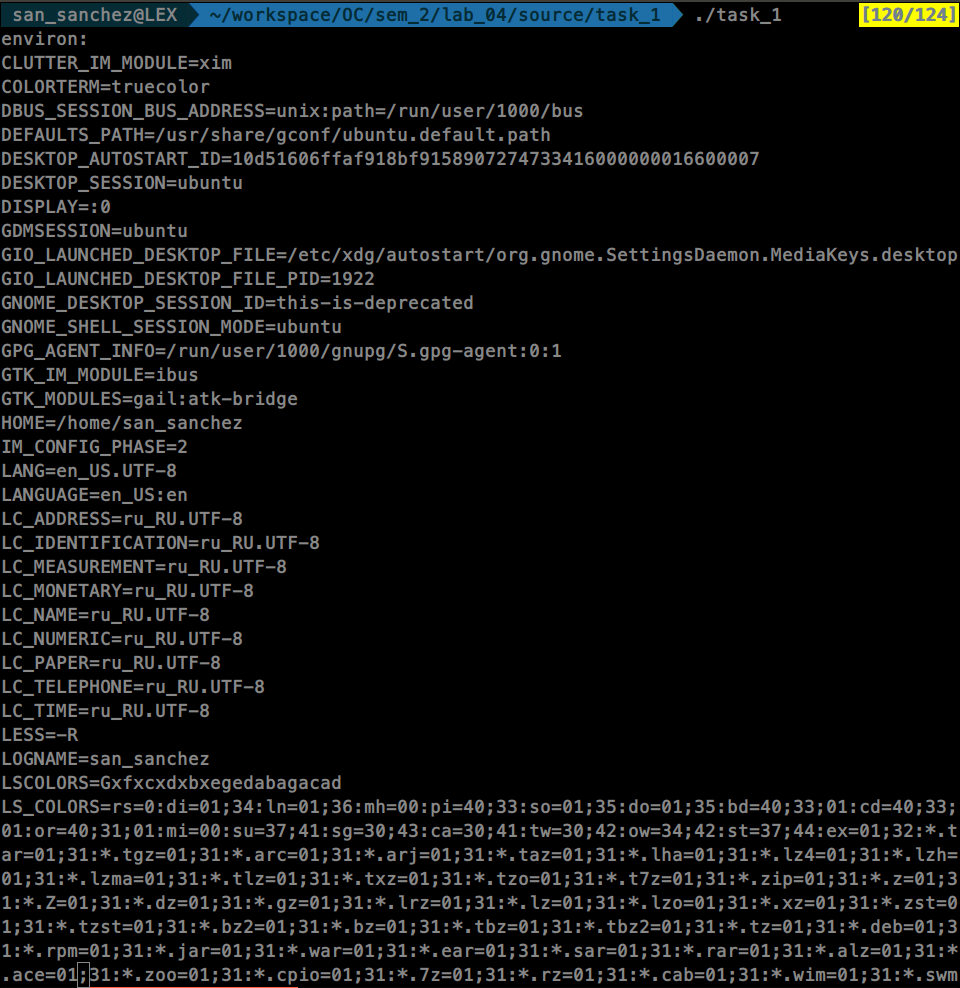
\includegraphics[scale=0.45]{data/image/env_1.png}
    \caption{Скришот вывода информации об окружении процесса (часть 1).}
\end{figure}

\begin{figure}[H]
    \centering
    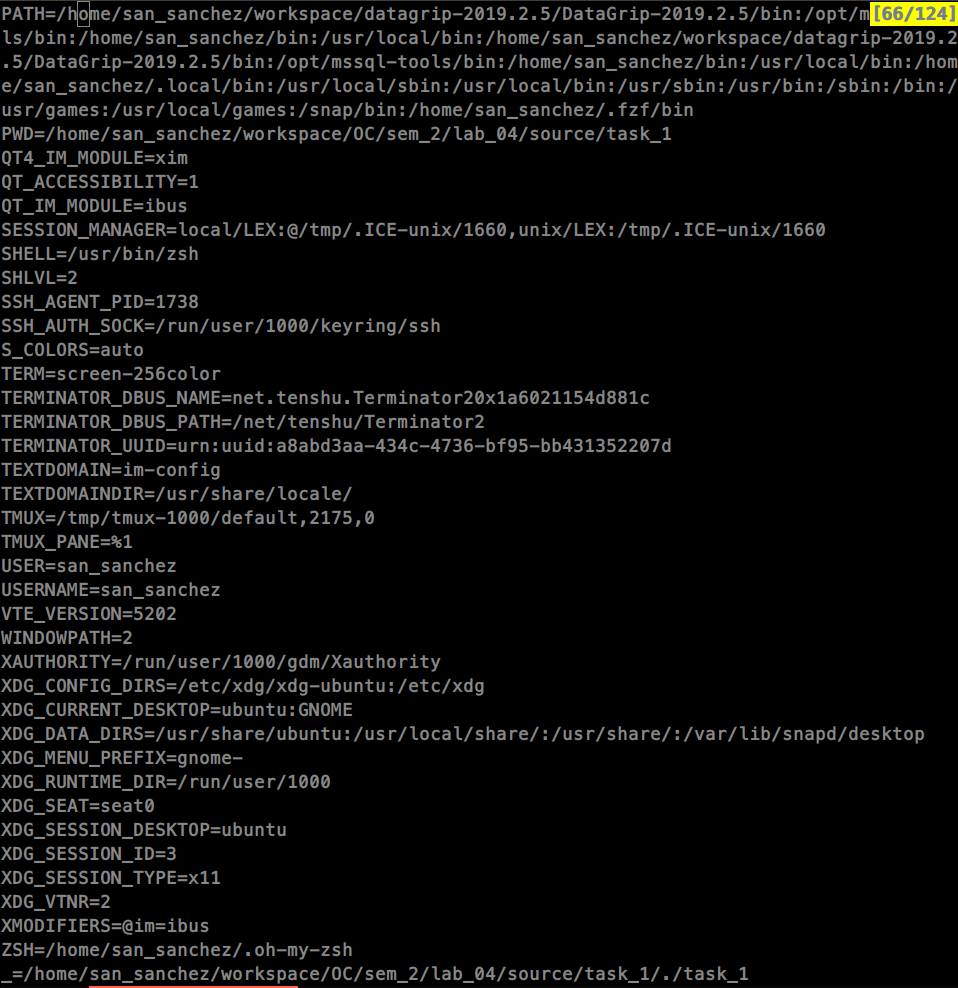
\includegraphics[scale=0.45]{data/image/env_2.png}
    \caption{Скришот вывода информации об окружении процесса (часть 2).}
\end{figure}

\begin{figure}[H]
    \centering
    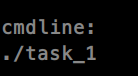
\includegraphics[scale=0.5]{data/image/cmdline.png}
    \caption{Скришот вывода содержимого файла cmdline.}
\end{figure}

\begin{figure}[H]
    \centering
    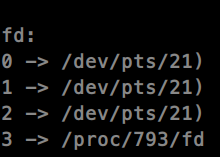
\includegraphics[scale=0.45]{data/image/fd.png}
    \caption{Скришот вывода содержимого директории fd.}
\end{figure}

\begin{figure}[H]
    \centering
    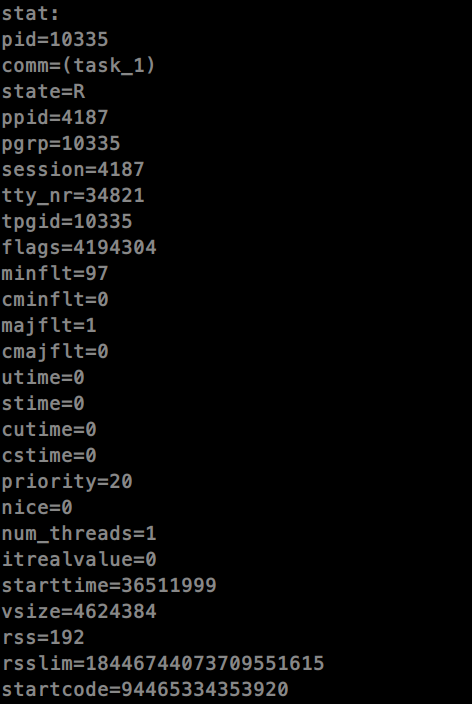
\includegraphics[scale=0.45]{data/image/stat_1.png}
    \caption{Скришот вывода состояния процесса. (часть 1)}
\end{figure}

\begin{figure}[H]
    \centering
    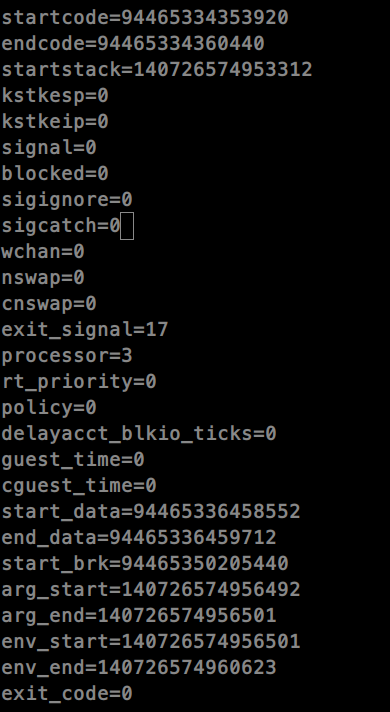
\includegraphics[scale=0.45]{data/image/stat_2.png}
    \caption{Скришот вывода состояния процесса. (часть 2)}
\end{figure}

\section{Задание \No{}2}
Написать программу – загружаемый модуль ядра (LKM) – которая поддерживает чтение из пространства пользователя и запись в пространство пользователя из пространства ядра.

\lstset{language=c}
\begin{lstlisting}[caption=Текст программы второго задания]
#include <linux/module.h>
#include <linux/kernel.h>
#include <linux/proc_fs.h>
#include <linux/string.h>
#include <linux/vmalloc.h>
#include <linux/fs.h>
#include <linux/uaccess.h>

MODULE_LICENSE("GPL");
MODULE_AUTHOR("Kupry");

static struct proc_dir_entry *proc_entry;
static struct proc_dir_entry *proc_dir;
static struct proc_dir_entry *proc_link;

static char *buffer;
static int buf_index, next_fortune;

static ssize_t fortune_write(struct file *filp, const char __user *buf, size_t len, loff_t *offp);
static ssize_t fortune_read(struct file *filp, char __user *buf, size_t count, loff_t *offp);

static int fortune_init(void)
{
    static struct file_operations fileops =
    {
        .owner = THIS_MODULE,
        .read = fortune_read,
        .write = fortune_write
    };

    buffer = (char *)vmalloc(PAGE_SIZE);
    if (!buffer)
    {
        printk(KERN_ERR "fortune: no memory for create buffer\n");
        return -ENOMEM;
    }

    memset(buffer, 0, PAGE_SIZE);

    proc_entry = proc_create("fortune", 0644, NULL, &fileops);
    if (proc_entry == NULL)
    {
        vfree(buffer);
        printk(KERN_ERR "fortune: couldn't create proc entry\n");
        return -ENOMEM;
    }

    proc_dir = proc_mkdir("fortune_dir", NULL);
    if (!proc_dir)
    {
        vfree(buffer);
        printk(KERN_ERR "fortune: Couldn't create proc dir, symlink\n");
        return -ENOMEM;
    }

    proc_link = proc_symlink("fortune_symlink", NULL, "/proc/fortune_dir");
    if (!proc_link)
    {
        vfree(buffer);
        printk(KERN_ERR "fortune: Couldn't create proc dir, symlink\n");
        return -ENOMEM;
    }

    buf_index = 0;
    next_fortune = 0;

    printk(KERN_INFO "fortune: module loaded.\n");
    return 0;
}

static ssize_t fortune_read(struct file *filp, char __user *buf, size_t count, loff_t *offp)
{
    if (*offp > 0)
    {
        return 0;
    }

    if (next_fortune >= buf_index)
    {
        next_fortune = 0;
    }

    count = copy_to_user(buf, &buffer[next_fortune], count);
    next_fortune += count;
    *offp += count;

    return count;
}

static ssize_t fortune_write(struct file *filp, const char __user *buf, size_t len, loff_t *offp)
{
    int available_space = PAGE_SIZE - buf_index + 1;

    if (len > (size_t)available_space)
    {
        printk(KERN_NOTICE "fortune: there isn't enough memory\n");
        return -ENOSPC;
    }

    if (copy_from_user(&buffer[buf_index], buf, len))
    {
        printk(KERN_NOTICE "fortune: copy_to_user failed\n");
        return -EFAULT;
    }

    buf_index += len;
    buffer[buf_index - 1] = 0;

    return len;
}

static void fortune_exit(void)
{
    proc_remove(proc_entry);
    proc_remove(proc_dir);
    proc_remove(proc_link);

    vfree(buffer);

    printk(KERN_INFO "fortune: module unloaded.\n");
}

module_init(fortune_init);
module_exit(fortune_exit);
\end{lstlisting}

~\

Результат:
\begin{figure}[H]
    \centering
    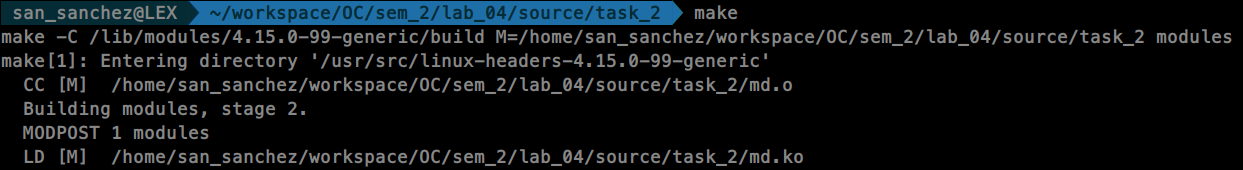
\includegraphics[scale=0.35]{data/image/task_2_1.png}
    \caption{Скришот сборки модуля.}
\end{figure}

\begin{figure}[H]
    \centering
    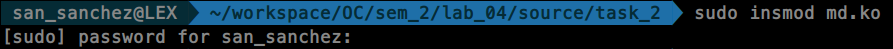
\includegraphics[scale=0.4]{data/image/task_2_2.png}
    \caption{Скришот загрузки модуля.}
\end{figure}

\begin{figure}[H]
    \centering
    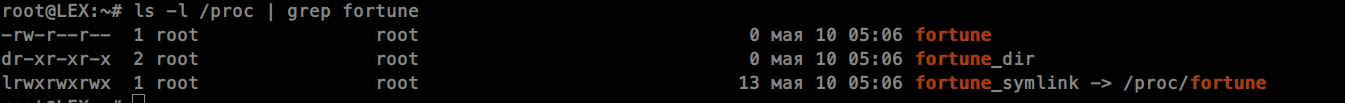
\includegraphics[scale=0.35]{data/image/task_2_cor_1.png}
    \caption{Скриншот созданных директории, файла и символьной ссылки.}
\end{figure}

\begin{figure}[H]
    \centering
    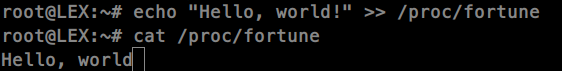
\includegraphics[scale=0.4]{data/image/task_2_4.png}
    \caption{Скриншот работы файла.}
\end{figure}

\begin{figure}[H]
    \centering
    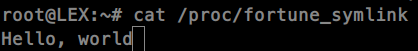
\includegraphics[scale=0.4]{data/image/task_2_cor_2.png}
    \caption{Скриншот работы ссылки.}
\end{figure}
